% Experiments

This section presents the experiments and results aimed at evaluating our proposed graph generative model. First we run a grid-search on the hyperparameter space to find the optimal configuration of the RGVAE. We use the ELBO and MRR as evaluation metric. The best configurations are used to perform link prediction. Here we compare the model performance with vs. without convolutions. We use the VDistMult as control model for link prediction. Finally we run two proof-of-concept experiments. The first generating triples and filter on a entity class constraining relation, thus we get an insight of how much percent of the generated triples are valid. Secondly we analyze the results of a RGVAE trained on subgraphs with $n=10$. For the experiments we use two multi-relational KG datasets.

% We covered link and node prediction and compared those to SOTA scores. Further we ran experiments on investigating the coherence of the reproduced graph structure. Lastly we measured the adherence of our model to the KG's underlying syntax.


\subsection{Data}
\label{ssec5:data}
For this sake of comparison with state of the art results, we chose the two most popular dataset used in this field of KG link prediction, FB15k237 and WN18rr.

% Training models on each dataset for 333 epochs, without early stopping.

\textbf{Fb15k-237}

textwidth for figures:
\printinunitsof{in}\prntlen{\textwidth}

linewidth for figures:
\printinunitsof{in}\prntlen{\linewidth}

Entity types

triple topics

% This dataset is a subset of the FreeBase KG (cite).[Explain Free Base] The original Fb15k had redundant triples, creating ambiguity during training. In the updated version, Fb15k-237, these triples were removed what led to a more robust dataset, which is commonly used as benchmark for several NLP tasks.

% % or/and
% A subset from one of the first and largest KGs, called FreeBase. In the first version of this dataset, it was possible to infer most of the test triples by inverting triples in the trainset, Thus the latest $237$ version filtered these triples out.
% The dataset contains $14,951$ entities and $1,345$ different relations.

\textbf{WN18rr}

Based on the wordnet KG.

Only $18$ different relations

triples are synsets (synonym, hypernym)

TODO Table comparing numbers

\subsection{Hyperparameter Tuning}

In this section we run a grid search for the three hyperparameters $\beta$, $d_z$ and $d_h$ for a set of contrastive values. To reduce the computational expenses we train each model for $60$ epochs and  evaluate link prediction on a subset of $50$ triples.

Empirically we set the learning rate to $3e-5$ and the maximum batchsize fitting on the GPU memory. For $d_h$ we did not see any significant changes for higher values, thus we choose a lower number to reduce the total model parameters. The remaining hyperparameter did influence and the optimal setting vary for each dataset, table \ref{tab:RGVAEhyp} shows the results of our hyperparameter tuning.

% lr empirically and batchszize fixed.

% beta
For the hyperparameter tuning of $\beta \in [0,1,10,100]$ we chose significant values. With $\beta = 0$ we do not constrain our model on the Gaussian prior, thus the latent distribution can take the form of any distribution. This reduces the influence of the variational module and the model becomes closer to an autoencoder. For $\beta = 1$ we get our base model, and for $\beta \in [10,100]$ the $\beta-$VAE version.


\begin{figure}[H]
    \centering
    \begin{subfigure}{.5\textwidth}
      \centering
      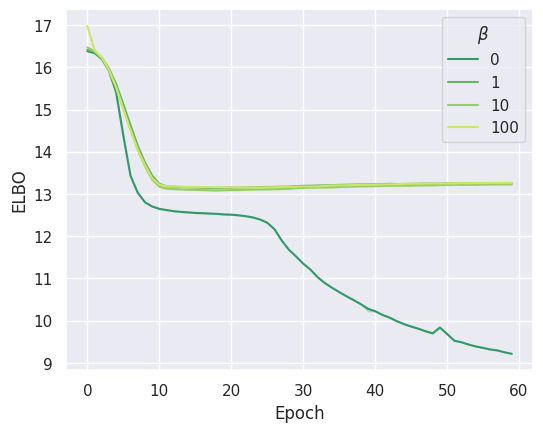
\includegraphics[width=.9\linewidth]{graphs/plots/beta_loss_fb.png}
      \caption{FB15K-237}
      \label{fig5:betafb}
    \end{subfigure}%
    \begin{subfigure}{.5\textwidth}
      \centering
      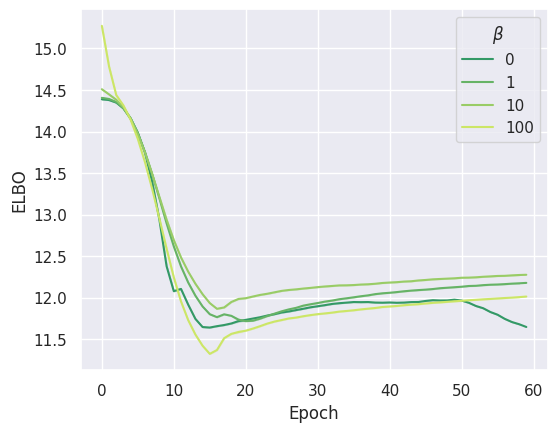
\includegraphics[width=.9\linewidth]{graphs/plots/beta_loss_wn.png}
      \caption{WN18RR}
      \label{fig5:betawn}
    \end{subfigure}
    \caption{Validation loss for RGVAE with $\beta \in [0,1,10,100]$ trained on each dataset.}
    \label{fig5:beta}
\end{figure}


Figure \ref{fig5:beta} shows the validation ELBO for the different $\beta$ values and for both datasets. We notice two interesting outcomes.  

\begin{enumerate}
    \item For $\beta = 0$ converges further than the rest.
    \item The remaining values behave quase identical with $\beta = 100$ performing slightly better. 
\end{enumerate}

Since setting $\beta = 0$ would undermine our hypothesis of evaluating variational model, we chose $\beta = 100$ as default for the following experiments. This also compares with the $\beta$ values proposed by Higgins in \cite{higgins_beta-vae_2016} to achieve a factorization of the latent space.

Especially on the FB15k-237 dataset the $\beta = 0$ configuration converges to a much lower ELBO. Thus, we have the trained models perform link-prediction on a $1\%$ subset of the validation set. The barplot \ref{fig5:betafbmrr} indicates an inverse correlation between the ELBO and the MRR score. 

\begin{figure}[H]
    \centering
      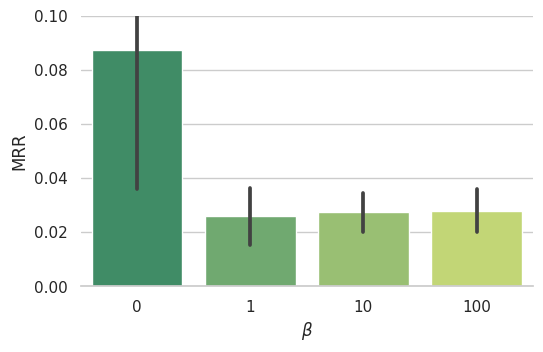
\includegraphics[width=.45\textwidth]{graphs/plots/beta_mrr_fb.png}
      \caption{MRR scores for different $\beta$ values on the dataset FB15k-237.}
      \label{fig5:betafbmrr}
\end{figure}

Barplot IN APPENDIX  

% d_z
Experiments on the impact of $d_z$ on the ELBO show little improvement for $10<d_z<100$ and from $100<d_z<1000$ insignificant to no improvement. Thus, we chose $d_z=100$ as default for our experiments.


% d_h did not influcence
Lastly, we evaluate the models hidden dimensions $d_h$ and its influence on the ELBO and the (subset)MRR. We compare between $d_h\in [256, 512, 1024, 2048]$, while the lowest configuration performs slightly worse on the ELBO, there is no significant difference between the remaining three configurations. Considering the models parameter count we chose the $d_h=512$ as default.


\subsection{Link Prediction}


 We now get to the main experiment of this thesis. The results of this experiment will show if the RGVAE architecture is suitable for link prediction and in first place, if it is able to grasp the underlying KG semantics at least significantly better than random by differentiating between real and corrupted triples. First we evaluate the performance of the RGVAE on this experiment, comparing both encoder versions. Then we investigate the influence of the variational inference by comparing the variational and original versions of DistMult on link prediction.
 
 \subsubsection{RGVAE}

 At this point we bring in the convolutional variation of our model, which we will denote as RGCVAE. The experiments reveal if the convolutional architecture holds an advantage compared to the simple MLP baseline. Further a randomly initiated and untrained RGVAE is used as control model.
 
 Due to its sparse graph computation, the RGVAE takes about 7 days to evaluate link prediction on the full test set and even 3 days when prediction tasks run parallel on a node of $4$ Nvidia Titan RX 25GB GPUs. Since the exemplary link prediction during experimenting with different hyperparameter already gave us an idea of the mediocre performance of our model, we chose to spare computation time and power by running link prediction on a randomly drawn one-third of the complete test set. Each run is repeated three times using a different random seed.

The results are visualized in figure \ref{fig5:lp_final}. We chose a visualization over a table, to emphasize our observations, and for the mentioned limitation of the test set, which makes these results not suitable for academically valid comparisons. Note that the figures are scales and to a range $[0,10]$ while all metrics have a maximum of $1$.

Comparing a MRR of $0.08$ to the DistMult score or $0.4$ our model does not perform competitively on link prediction tasks.

% Better than random?? I hope so.

Graph convolutions do not yield an advantage over the basemodel. In fact, the RGVAE with convolutions even scores slightly worse. 

%  FOR Conclusion: this might be because of the implementation of stacking the matrices.
The model scores about three times better on the FB15k-237 dataset than on WN18RR. FB15k-237 is a richer dataset with more triples and and a more balanced ratio of entities to relations. WN18RR operates on only 18 relations, what makes the relation most crucial when completing a triple. The architecture of the RGVAE puts twice the emphasis entities, described by the adjacency and the node feature matrices, while the relation is only represented by the overly sparse edge attribute matrix. Thus, we could conclude that our model learns to predict based on the hidden types and topics of the entities. All possible conclusions for this are discussed in \ref{sec:discus}. Relevant for this section is solely, that we chose the FB15k-237 dataset to investigate further, how well the RGVAE's grasps the underlying entity types and triple topics.   

%  REASON: fb has more relations, is a more complete KG. wn only 12 relations and more entities. Model emphasizes entities (adj and node features), relations may be less relevant, wn is more about the relation (same/ not the same). This indicates that our model grasps the hidden types and topics of the FB entities.


 \begin{figure}[H]
  \centering
  \begin{subfigure}{.5\textwidth}
    \left
    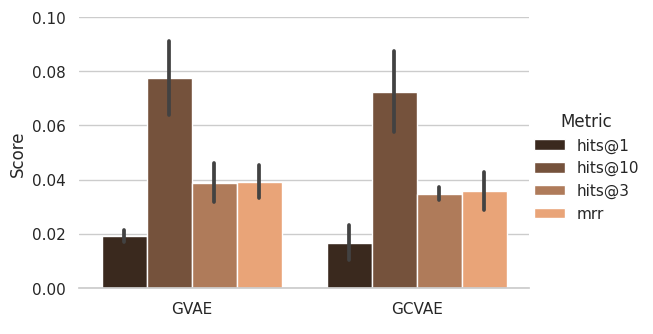
\includegraphics[height=.5\textwidth, keepaspectratio]{graphs/plots/lp_fb.png}
    \caption{FB15K-237}
    \label{fig5:lpfb}
  \end{subfigure}%
  \begin{subfigure}{.5\textwidth}
    \right
    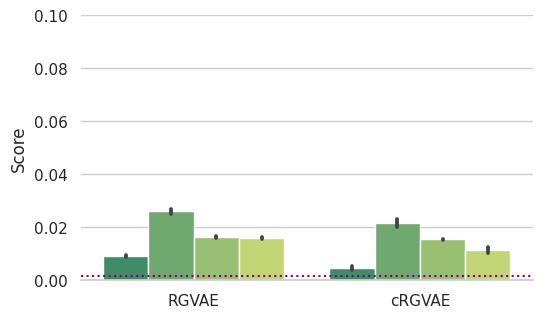
\includegraphics[height=.5\textwidth]{graphs/plots/lp_wn_wol.png}
    \caption{WN18RR}
    \label{fig5:lpwn}
  \end{subfigure}
  \caption{Link prediction results in MRR, Hits@1, Hits@3 and Hits@10 for RGVAE and RGCVAE trained on the full trainset of each dataset.}
  \label{fig5:lp_final}
\end{figure}

TODO add random!!!

% Compare with vs without convolution 
% We use negative elbo as scoring function. Since elbo is aimed to be reduced and LP scores are higher better.

% We try with and without permutation

% We try the model as encoder only NO

% We use 1/3 of the test set only, randomly drawn. Run 3 times?
% Final models only 60 epochs


\subsubsection{DistMult}

In order to explain the poor performance of the RGVAE on the task of link prediction, we investigate th impact of the variational inference. Since the RGVAE with relaxed latent space, meaning less variance, indicated higher scores than the version with Gaussian prior, we examine the two variants by means of embedding models. The original DistMult model with optimized parameter serves as control model, while we compare it to the VDistmult, described in section \ref{ssec4:vdistm}, learning the full ELBO versus learning only on the reconstruction loss. By not including the regularization term in the loss the model is no longer bound to the Gaussian prior, which results in a relaxation of the latent space.

We train the three models for $300$ epochs solely on the FB15k-237 dataset and evaluate MRR, Hits@$1$, Hits@$3$ and Hits@$10$. Table \ref{tab5:VarDistM} shows the scores with $\mu \pm \sigma$ of three runs per model. Note that the exponent on $\sigma$ holds for the whole term. We can clearly see that both variational versions of the DistMult perform significantly worse than the original model. Learning on the full elbo or only the reconstruction loss does not seem to influence the scores in this setting. This indicates, that the models performance on link prediction suffers from using variational inference.

% TODO: Answer question:Link prediction with control model:

% Trained for 300 epochs

% We see that the variational part messes everything up.

% Table:
% MRR + Hits@all + Loss

\begin{table}[H]
  \centering
      \begin{tabular}{|l|l|l|l|l|}
      \hline
      \rowcolor[HTML]{EFEFEF}
      \multicolumn{1}{|c}{\textsc{DistMult ver.}} & \multicolumn{1}{c}{\textsc{MRR}} & \multicolumn{1}{c}{\textsc{Hits@$1$}} & \multicolumn{1}{c}{\textsc{Hits@$3$}} & \multicolumn{1}{c|}{\textsc{Hits@$3$}} \\\hline
      Original     & \multicolumn{1}{c|}{$0.2854\pm 0.0025$} & \multicolumn{1}{c|}{$0.2\pm 0.001$} & \multicolumn{1}{c|}{$0.3149\pm 0.0038$} & \multicolumn{1}{c|}{$0.4512\pm 0.0053$}  \\
      Variational   & \multicolumn{1}{c|}{$0.5170\pm 0.0197e^{-3}$} & \multicolumn{1}{c|}{$0.2442\pm 0.1994e^{-4}$} & \multicolumn{1}{c|}{$0.8145 \pm 0.3049e^{-4}$} & \multicolumn{1}{c|}{$0.3990\pm 0.05760e^{-3}$} \\
      Var. w/ ELBO   & \multicolumn{1}{c|}{$0.6397\pm 0.0357e^{-3}$} & \multicolumn{1}{c|}{$0.5700\pm 0.3046e^{-4}$} & \multicolumn{1}{c|}{$0.1547\pm 0.1023e^{-3}$} & \multicolumn{1}{c|}{$0.6351\pm 0.1992e^{-4}$} \\
      \hline
      \end{tabular}
      \caption{Link prediction scores of DistMult versions on the FB15k-237 dataset.}
      \label{tab5:VarDistM}
  \end{table}


\subsection{Impact of permutation}
% Check if adj matrix adheres to edge attribute matrix.

TODO

Permutation starts at $100\%$ at the beginning of training and converges to $60\%$.

Model without predicts adj node always in the upper right just as the target. Model with predicts much more variations of adjacency.

Graph of permutation during training.
loss with vs without 

\subsection{Interpolate Latent Space}

TODO

We take two random triples and interpolate the latent space of these two triples. The interpolations result in: HERE AN EXAMPLE.

Further we go ahead and test what happens if we modify one latent dimension at a time with $d_z = 10$ of a triple. TABLE: (s,r,o), x_axis dims, y_axis steps. $95\%$ Gaussian confidence 

Can the model assign logical features to latent dimensions?


\subsection{Syntax coherence}

TODO

Check model trained with vs without perm invariance.

Check if generated triples follow basic logic.
\begin{itemize}
    \item Generate triples by random signals
    \item Filter these triples on type fixed relation
    \item Check if the entity is of this type.
\end{itemize}

Since there is no preset for how to check the semantics of a KG, we will use simple basic logical criteria.
The generated triples are filtered for the relation 'is capital of', thus the subject entity should be of type 'city' and the object entity of type 'country' and both adhere follow the topic 'location',
Curious if this gives good results.


\subsection{Subgraph Generation}

TODO

Until now our model trained on only one triple per sparse graph. What will happen if we train it on more than one triples?
